\documentclass
  [ams,pdfout]% class options
        {aesbr}
\RequirePackage[utf8]{inputenc}
\RequirePackage[english,brazil]{babel}
\RequirePackage{textcomp}
\RequirePackage{url}
\begin{document}
\begin{TitlePage}

  \Title{Produção de áudio com Web Audio}
  \RunningTitle{Produção de áudio com Web Audio}
  \RunningAuthors{Lunhani et al.}

  \Author
      [gcravista@gmail.com]
      {Guilherme Martins Lunhani}
      \Affil
          [A]
          {
            LabMacambira.sf.net,
            São Carlos, SP, Brasil
          }
          \Author
              [vilson@void.cc]
              {Vilson Vieira}
              \Affil
                  [B]
                  {
                    Universidade de São Paulo,
                    Instituto de Física de São Carlos,
                    Departamento de Física Computacional,
                    São Carlos, SP, Brasil
                  }
          \Author
              [ricardo.fabbri@gmail.com]
              {Ricardo Fabbri}
              \Affil
                  [C]
                  {
                    Universidade do Estado do Rio de Janeiro,
                    Instituto Politécnico,
                    Departamento de Modelagem Computacional,
                    Nova Friburgo, RJ, Brasil
                  }
          \Author
              [rfabbri@gmail.com]
              {Renato Fabbri}
              \Affilref
                  [B]

                  \Abstract{ Tecnologias Web têm se apresentado como
                    um catalisador para o uso criativo de mídias na
                    Internet. Embora essas tecnologias tenham sido
                    historicamente usadas em aplicações visuais, há
                    recentemente uma preocupação em desenvolver
                    interfaces para o processamento de áudio em
                    navegadores Web. Web Audio API é uma interface que
                    está sendo padronizada para o processamento de
                    áudio em tempo real na Web. Através dela é
                    possível desenvolver aplicações que vão desde
                    sistemas de composição musical em tempo real até
                    mixers distribuídos e colaborativos, sem a
                    necessidade da instalação de plugins proprietários
                    ou configurações complexas. Procurando contribuir
                    para o desenvolvimento desta tecnologia,
                    introduzimos a Web Audio API através de exemplos
                    simples, na forma de um tutorial e apresentamos
                    aplicações que foram desenvolvidas utilizando essa
                    tecnologia.  }
\end{TitlePage}

\section{INTRODUÇÃO}

Recentemente observamos um encorajamento no desenvolvimento de
bibliotecas dedicadas ao processamento de áudio digital em navegadores
da \emph{internet}(Web Audio API)~\cite{webaudio}, o que viabilizou
projetos como
dataflow-webaudio\footnote{http://forresto.github.com/dataflow-webaudio/,
  acessado em fevereiro de 2013} e
Mix.js\footnote{http://kevincennis.com/mix/, \emph{ibd.}}. No Brasil,
o grupo LabMacambira.sf.net\footnote{Grupo de desenvolvedores de
  software livre, http://labmacambira.sourceforge.net/, ibd.} conta
com experimentos como
Vivace~\cite{Vivace,foobarbaz}\footnote{https://github.com/automata/vivace}. Este
último é uma proposta de \emph{live
  coding}\cite{nilson2007live,collins2003live,ward2004live,collins2011live},
no qual é realizada uma performance artística junto a um público, onde
intérpretes editam e executam códigos de programação utilizados para
processar materiais sonoros e visuais \emph{in live}.

Processos de \emph{criação}, \emph{edição} e \emph{mixagem} são
transformados com uso de \emph{aplicativos web}; neste artigo faremos
uma breve descrição técnica da Web Audio API, das ferramentas
desenvolvidas, e reflexões de seus usos em atividades de produção
musical.

\section{CRIAÇÃO, EDIÇÃO E MIXAGEM: UMA REVISÃO DE CONCEITOS E FERRAMENTAS}

Os campos de produção musical e visual compartilham destes termos,
onde cada um possui conceitos, ferramentas e técnicas próprias. Neste
trabalho trataremos daqueles da produção musical, assim como explanado
por \cite{izhaki2008mix} (Figura~\ref{figure:mix_chain}).

\begin{figure}[htpb]
  \begin{center}
    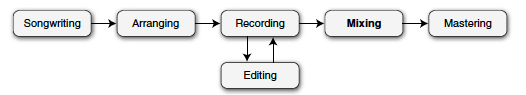
\includegraphics[scale=.4]{../img/mix_chain.png}
    \caption{Etapas do processo de produção musical (retirado de
      \cite{izhaki2008mix})}
    \label{figure:mix_chain}
  \end{center}
\end{figure}

Criação, edição e mixagem são etapas separadas; o primeiro pode
adquirir facetas individuais, enquanto editar e mixar podem se
apresentar como:

\begin{itemize}
    \item edição seletiva: processo de seleção dos materiais sonoros
      mais adequados, bem como o processo de combinar os materiais
      escolhidos em um \emph{take} mestre~\cite{izhaki2008mix}.
    \item edição corretiva: processo onde se corrige partes
      defeituosas dos materiais escolhidos, que podem ter causas
      diversas: má performance do intérprete, captação inadequada,
      entre outros.
    \item mixagem: Uma etapa do processo de produção musical no qual
      os materiais - amostrados ou sintetizados - são balanceados,
      tratados e combinados entre si em um formato multicanal, mais
      comumente em estereo de dois canais.
\end{itemize}

Em grandes estúdios essas etapas se dividem entre o compositor,
arranjador, produtor musical e engenheiros de som. De maneira bastante
superficial, os dois últimos utilizam um computador com
\emph{softwares}(como ProTools, Logic, Nuendo), que pode conter etodas
as ferramentas de edição e mixagem.

Acreditamos que com ferramentas \emph{Web} podemos agrupar as três
etapas em questão \footnote{Essas três atividades agrupadas é algo que
  experenciamos durante o \emph{live coding}: o código-fonte é
  interpretado pelo computador e logo em seguida transformado em
  material sonoro por processamento de áudio digital (DSP)} e
sociabilizar a produção musical. A criação deixa de ser individual, a
edição deixa de ser apenas seletiva ou corretiva, a mixagem deixa de
ser apenas uma maneira de balançear os materiais, uma vez que todos
podem influenciar em qualquer parte do processo de produção.

\section{WEB AUDIO}

Historicamente as tecnologias Web estiverem focadas em aplicações
gráficas. O design de interfaces com o usuário era até então
prioridade. Recentemente, a necessidade pela manipulação de mídias fez
surgir APIs implementadas diretamente em navegadores Web, que oferecem
a possibilidade de manipular áudio e vídeo em tempo real, através de
JavaScript. Com o desenvolvimento da versão 5 do padrão HTML, houve a
criação de métodos e modelos para manipulação de imagens (através de
procedimentos em JavaScript que permitem processar pixel a pixel a
matriz de uma imagem, inserida em uma \emph{tag} $<canvas>$), vídeos
(por procedimentos que manipulam \emph{tags} $<video>$) e áudio
(\emph{tags} $<audio>$).

Porém, aplicações como a síntese e demais operações de processamento
de áudio em tempo real não eram possíveis, mesmo usando tais
\emph{tags}. A única forma de se processar áudio em tempo real era
através do uso de plugins proprietários como
\emph{Flash}. Recentemente, David Humphrey e colaboradores iniciaram o
desenvolvimento de APIs que permitem acesso direto à interface de
áudio a partir do browser. A primeira implementação de uma API deste
tipo ficou conhecida como Audio Data API~\cite{audiodata},
implementada no navegador Mozilla Firefox. Com esse esforço e o
reconhecimento da comunidade Web da necessidade de APIs para
processamento de áudio em navegadores, o consórcio W3 criou um grupo
de trabalho que terminou com o desenvolvimento de uma API padrão para
processamento de audio. Essa API ficou conhecida como Web Audio.

Web Audio é escrita em código nativo (C++ e Assembly) para garantir
performance máxima no processamento de áudio em navegadores
\emph{Web}\footnote{Atualmente, poucos navegadores tem suporte
  completo e utilizamos aquele distribuido pelos desenvolvedores
  \emph{WebKit} (i.e. \emph{Safari} e \emph{Chromium}. Uma
  implementação para o navegador Mozilla Firefox está em atual
  desenvolvimento.}. É baseada no paradigma de \emph{grafos de
  unidades de áudio}, onde se especifica uma coleção de nós e rotinas
de conexão e desconexão entre eles (Figura \ref{figure:graph}). Entre
algumas de nossas motivações com Web Audio API, estão a síntese,
ganho, equalização, expansão multicanal (estereofonia de 2.0 e 5.1
canais) e efeitos (reverb). Ainda, através da Web Audio API podemos
tocar um arquivo de áudio (ou \emph{buffers} sintetizados em tempo
real por osciladores) em um tempo qualquer, com precisão, além de
poder acessar amostras de áudio para análise espectral, por exemplo.

\subsection{Síntese e sampling}

Afim de ressaltar a facilidade do uso de Web Audio para a criação de
aplicações Web para processamento de áudio, apresentamos aqui um breve
tutorial de seu uso.

Antes de fazer qualquer operação de processamento de áudio, devemos
criar um \emph{contexto}. Ali o áudio será processado~\footnote{O
  conceito de contexto foi inserido em Web Audio para ser compatível
  com o contexto $<canvas>$ do padrão HTML5}. Criamos um contexto
através das seguintes instruções:

\begingroup
    \fontsize{8pt}{9pt}\selectfont
\begin{verbatim}
var contexto = new webkitAudioContext();
\end{verbatim}
\endgroup

Não há a necessidade de se criar mais de um contexto de áudio para uma
mesma página Web. É importante notar que o prefixo \emph{webkit} usado
no construtor da classe \emph{AudioContext} é utilizado
provisoriamente, até não se ter um padrão único em uso por todos os
navegadores.

Após a criação do contexto, podemos criar um \emph{buffer} de áudio
para podermos ler arquivos de áudio a partir de um servidor Web remoto
ou de arquivos enviados localmente pelo visitante da página. É uma
prática comum carregar os arquivos de áudio logo na inicialização da
página, pois assim evitamos atrasos na execução. Todo o \emph{buffer}
de áudio é não-persistente, e portanto, podemos refazer sua leitura no
momento que desejarmos e quantas vezes forem necessárias, sem termos
de reler o arquivo de áudio.

O carregamento de um arquivo de áudio é feito através de uma
requisição assíncrona por HTTP. Desta forma, fazemos um pedido ao
servidor Web para abrir o arquivo de áudio especificado (no caso do
exemplo a seguir, o arquivo de nome \emph{foo.wav}) e informamos uma
função (\emph{insereNoBuffer}) que irá ler o arquivo em um
\emph{buffer}. A requisição é dita assíncrona pois o processo
principal de JavaScript não ficará em um estado de espera até o
arquivo ser lido e armazenado em \emph{buffer}.

\begingroup
    \fontsize{8pt}{9pt}\selectfont
\begin{verbatim}
requisicao = new XMLHttpRequest();

requisicao.open('GET', 'foo.wav', true);

requisicao.responseType = 'arraybuffer';

requisicao.addEventListener('load', 
   insereNoBuffer, false);

requisicao.send();
\end{verbatim}
\endgroup

A função \emph{insereNoBuffer}, por sua vez, recebe a requisição e
cria um \emph{buffer} fazendo uma chamada ao contexto (todos os
métodos e construtores para processamento de áudio são acessíveis a
partir do contexto). Por fim, uma variável é usada para referenciar o
\emph{buffer}.

\begingroup
    \fontsize{8pt}{9pt}\selectfont
\begin{verbatim}
var fonte;

function insereNoBuffer(evento) {
    var req = evento.target;

    var bufFonte = 
   contexto.createBufferSource();

    bufFonte.buffer = 
   contexto.createBuffer(req.response, false);

    fonte = bufFonte;
}
\end{verbatim}
\endgroup

O processo de se requisitar, ler e inserir em \emph{buffer} é
certamente a operação mais complexa e prolíxa. As demais operações
possuem uma interface bastante intuitiva e familiar a engenheiros de
áudio, por se basear em grafos de unidades.

Além de carregar um arquivo de áudio, é possível sintetizar ondas
comuns através de osciladores.

\begingroup
    \fontsize{8pt}{9pt}\selectfont
\begin{verbatim}
var fonte = contexto.createOscillator();

fonte.type = 0;
\end{verbatim}
\endgroup

Neste caso estamos criando uma onda senoidal, pois especificamos seu
tipo como $0$. Podemos ainda criar os tipos de onda quadrada, dente de
serra e triangular, que possuem os identificadores 1, 2 e 3,
respectivamente.

Após termos criado nossa \emph{fonte} de áudio, seja inicializando-o
com amostras de um arquivo ou sintetizadas por um oscilador, podemos
executá-lo. Para tal, devemos conectá-lo a um \emph{destino} no
contexto.

\begingroup
    \fontsize{8pt}{9pt}\selectfont
\begin{verbatim}
fonte.connect(contexto.destination);
\end{verbatim}
\endgroup

Para tocarmos o conteúdo da \emph{fonte}, usamos o método
\emph{noteOn}, especificando o tempo (em segundos) quando deverá ser
tocado. No caso do exemplo a seguir, tocamos a \emph{fonte} no exato
momento da chamada do método.

\begingroup
    \fontsize{8pt}{9pt}\selectfont
\begin{verbatim}
buffer.noteOn(0);
\end{verbatim}
\endgroup

\subsection{Filtros e mixagem}

Por utilizar um paradigma baseado em grafos, a programação com Web
Audio torna-se facilitada e familiar ao engenheiro de áudio. Assim
como em um sintetizador modular, onde fios (ou \emph{cord patches})
são usados para ligar um módulo ao outro, podemos adicionar uma
infinidade de unidade de áudio entre uma \emph{fonte} e um
\emph{destino}, interligando-os da maneira que acharmos interessante
para nossos fins.

Um exemplo comum em processamento de áudio é utilizar um nó para
controle de volume, um filtro baseado em convolução e um compressor
para controle dinâmico do sinal sendo sintetizado. Em Web Audio,
criamos os nós fazendo chamadas a métodos com o prefixo \emph{create}
e armazemos referências a essas unidades que são em seguidas
conectadas umas as outras, e por fim, ao destino. Podemos então tocar
a fonte da maneira que desejarmos.

\begingroup
    \fontsize{8pt}{9pt}\selectfont
\begin{verbatim}
var compressor = 
   contexto.createDynamicsCompressor();

var reverb = 
   contexto.createConvolver();

var volume = contexto.createGainNode();


fonte.connect(compressor);

compressor.connect(reverb);

reverb.connect(volume);

volume.connect(contexto.destination);

fonte.noteOn(0);
\end{verbatim}
\endgroup

%\subsection{Análise espectral}

\section{APLICAÇÕES: USO DE WEB AUDIO PARA PRODUÇÃO MUSICAL}

Nessa seção abordamos aplicações que utilizam Web Audio para a
produção musical. Através da Web Audio API um novo horizonte de
possibilidades se abriu para o desenvolvimento de aplicações voltadas
para áudio. Por ser acessível através de uma interface concisa a
partir de JavaScript, pode ser usada em conjunto com outras
tecnologias Web (e.g.\ WebGL) para a criação de efeitos sonoros em
jogos, aplicações em visualização musical de forma criativa, sistemas
para produção musical com alta fidelidade.

Apresentamos aqui sistemas que foram implementados utilizando a Web
Audio API para a mixagem de áudio (Mix.JS), uma linguagem de dataflow
para manipulação multimídia (Dataflow-WebAudio) e um sistema para
composição em tempo real de um estilo de performance em Música
Eletroacústica conhecido como \emph{live coding} (Vivace), criado
pelos autores, e o qual abordamos em maiores detalhes.

\subsection{Mix.JS}

Desenvolvido por Kevin Ennis\footnote{http://www.kevincennis.com},
apresenta uma simples interface semelhante a uma mesa de som e um
playback da obra \emph{1901}, do grupo "Pheonix", como ilustrado na
Figura~\ref{fig:mixer}; apresenta uma \emph{pista} com amostras de
instrumentos diversos, controles de ganho, panoramização e
visualização do sinal de áudio em um \emph{VUmeter}. O usuário pode
experenciar a etapa de mixagem dos materiais já criados, gravados e
editados.

\begin{figure}[htpb]
  \begin{center}
    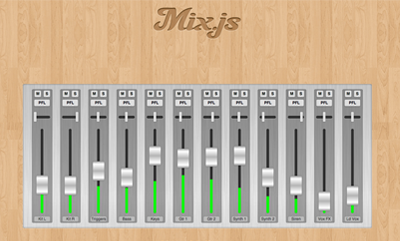
\includegraphics[scale=.4]{../img/mixer.png}
    \caption{Interface principal de Mix.JS}
    \label{fig:mixer}
  \end{center}
\end{figure}

\subsection{Dataflow-WebAudio}

Desenvolvido por Forrest Oliphant\footnote{http://forresto.com/},
apreenta uma interface de grafos (Figura~\ref{fig:dataflow}), onde
"caixas" são módulos de áudio e o usuário pode criar uma série de
combinações de roteamento entre eles. Se assemelha a \emph{softwares}
como Max/MSP e PureData.

\begin{figure}[htpb]
  \begin{center}
    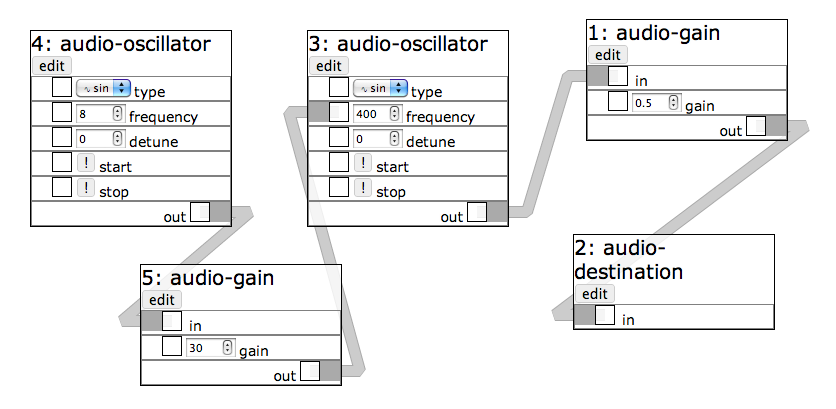
\includegraphics[scale=.2]{../img/dataflow.png}
    \caption{Dataflow utiliza caixas para manipular nós de áudio de
      Web Audio}
    \label{fig:dataflow}
  \end{center}
\end{figure}

\subsection{Vivace}

Desenvolvido pelo grupo LabMacambira, viabilizamos um espaço virtual
compartilhado como meio para edição e mixagem em performances
artísticas. Neste ambiente (Figura~\ref{figure:vivace}) pressupomos a
manipulação de \emph{vozes}, que são representações de amostras em
formato \emph{.wav} e/ou \emph{.mp4}. Com uso das tecnologias
\emph{Web Audio API, share.js e dat.GUI}, desenvolvemos um sistema
para edição e mixagem colaborativa.

\begin{figure}[htpb]
  \begin{center}
    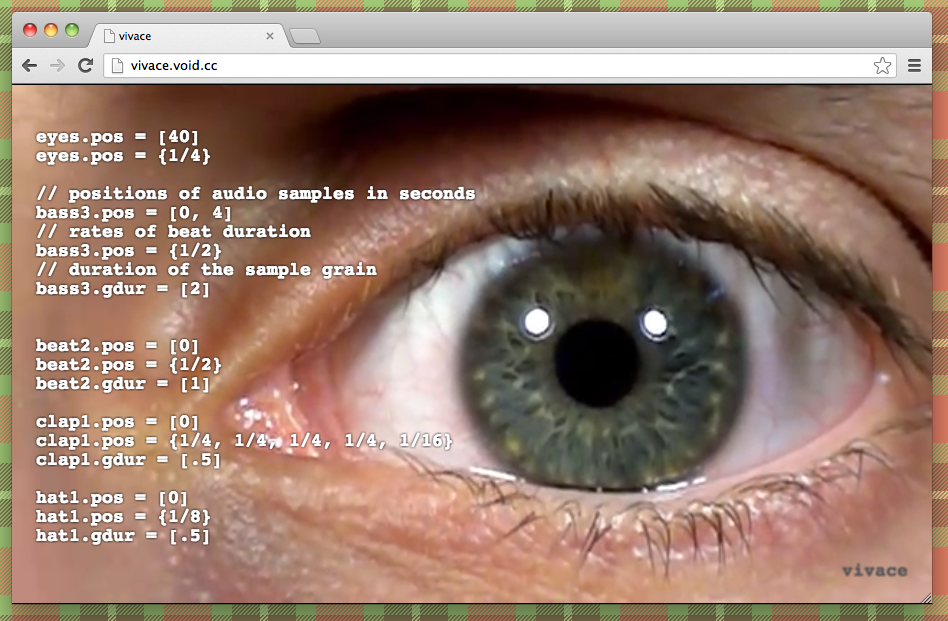
\includegraphics[scale=.2]{../img/fig_vivace.png}
    \caption{O ambiente Vivace}
    \label{figure:vivace}
  \end{center}
\end{figure}

A Figura~\ref{figure:vivace} apresenta:

\begin{itemize}
    \item Edição de um código-fonte (que chamaremos de vivace-lang),
      responsável pela manipulação dos materiais sonoros.
    \item Um mixer compactado com um controle básico de estereofonia
      (ganho, panoramização, equalizador de 3 bandas).
\end{itemize}

\subsubsection{Web Audio API e Vivace}

Na Figura~\ref{figure:graph} temos representado uma corrente de nós
para cada voz no Vivace. A estratégia utilizada para roteamento, foi
criar uma definição de um \emph{mixer} (com as propriedades
\emph{gain, pan, high, medium, low}) e aplicá-la através de uma
simples sintaxe de grafos:

\begingroup
    \fontsize{8pt}{9pt}\selectfont
\begin{verbatim}
# UMA DEFINIÇÃO DE UM MIXER
_mixerDef = function(){
   this.pan = 0
   this.compressor = 0
   this.reverbTime = 0.1
   this.gain = Math.sqrt(2)
   this.high = 2000
   this.Q_high = 0.5
   this.gain_high = 0
   this.medium = 2000
   this.Q_medium = 0.5
   this.gain_medium = 0
   this.low = 2000
   this.Q_low = 0.5
   this.gain_low = 0

# PROCESSO DE ROTEAMENTO (FEITO PARA CADA VOZ)
# PODEMOS ROTEAR NA FORMA: 
method = "source=>compressor=>
          reverb=>low=>medium=>
          high=>gain=>
          pan=>destination"
router('minhavoz', 
       new _mixerDef(), method)
\end{verbatim}
\endgroup

\begin{figure}[htpb]
  \begin{center}
    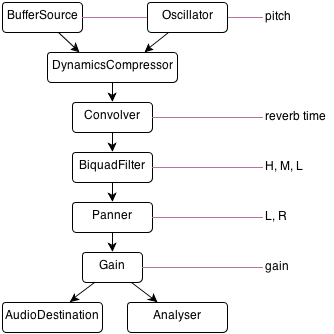
\includegraphics[scale=.4]{../img/fig_chain.png}
    \caption{Grafo de unidades de áudio e roteamento entre elas no Vivace}
    \label{figure:graph}
  \end{center}
\end{figure}


\subsubsection{Vivace-lang}

Vivace-lang é uma linguagem de domínio específico, parte do ambiente
Vivace. A criação de uma nova linguagem proporciona o uso de
construções sintáticas flexíveis que permitem produzir musicas de
maneira simples e mais familiar a músicos e até mesmo pessoas sem
treinamento musical ou computacional. Essa liberdade em se ter uma
linguagem que atenda à necessidades técnicas e artísticas permite uma
maior flexibilidade de improvisação. E a improvisação, por
conseguinte, encontra lugar comum nas práticas de \emph{live
  coding}. Ter uma linguagem de sintaxe simples, com poucas regras e
comandos, diminuem a ocorrência de erros durante a sessão.

Durante a edição do código vivace-lang, realizamos operações comuns na
prática de composição musical (reverter, inverter, transpor),
aplicadas aos \emph{frames} das amostras de áudio \cite{fabbri2013}:

No Vivace caracterizamos a essas amostras digitais, propriedades de
notas musicais. Canonicamente, as notas possuem ao menos duração,
volume, altura e timbre e são passíveis de serem
tratadas quantitativamente~\cite{fabbri2013}:

\begin{itemize}
    \item \emph{pos}: posições da amostra (no buffer da voz) a serem tocadas, em segundos.
    \item \emph{dur}: durações da amostra selecionada na voz, em
      segundos.
    \item \emph{gdur}: durações de cada grão sonoro, da voz, em segundos.
\end{itemize}

Esses valores podem ser \emph{literais}, \emph{operados} ou \emph{gerados}:

\begingroup
    \fontsize{8pt}{9pt}\selectfont
\begin{verbatim}
#CRIAÇÃO E EDIÇÃO
foo.pos = [1, 2, 3]
foo.pos = [.1, .2, .3] reverse                         
foo.pos = [1, 2, 3] inverse 
foo.pos = [1, 2, 3] transpose +2  
foo.dur = [2, 3, 4]  
foo.dur = [2, 3, 4] reverse 
foo.dur = [2, 3, 4] inverse
foo.dur = [2, 3, 4] transpose +1

# podemos gerar esses valores
foo.pos = [1/i+1 for i in [1, 2, 3]]

# ou combina-los com as operações
foo.dur = [1/i+1 for i 
           in [1, 2, 3]] reverse

#MIXAGEM
foo.amp = 1                                   
bar.amp = 0.5
baz.amp = 0.25

foo.pan = -1    #Esquerdo
bar.pan = 0    #centro
baz.pan = 1    #direito

foo.high = (freq: 2000, Q: 0.5, amp: 0.75)
bar.medium = (freq: 800, Q: 1, amp: 0.4)
baz.low = (freq: 200, Q: 0.5, amp: 0.67)
\end{verbatim}
\endgroup

\subsubsection{Vivace e dat.GUI}

Compreendemos também que este ambiente pode não ser totalmente
familiar a músicos ou engnehieos de som; utilizar apenas o vivace-lang
tornaria a experiência menos frutífera. Com o uso da biblioteca
dat.GUI\footnote{http://workshop.chromeexperiments.com/examples/gui/},
temos uma pequena interface gráfica que lembra uma mesa de som,
constituída de \emph{sliders}.

\begin{figure}[htpb]
  \begin{center}
    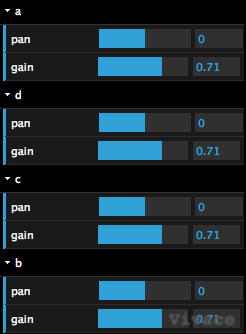
\includegraphics[scale=.4]{../img/datgui.png}
    \caption{interface gráfica do mixer em Vivace}
    \label{figure:vivace}
  \end{center}
\end{figure}

\section{CONCLUSÕES}

O uso de uma API como Web Audio permite a exploração de aplicações de
grande interesse para a engenharia de áudio, composição musical e
demais atividades que envolvam o processamento sonoro. Por sua
facilidade de programação, possibilita a prototipação de aplicações
sonoras, novos instrumentos e experimentações em Música
Eletroacústica.

Apresentamos a API através de exemplos de simples compreensão e
aplicações que foram desenvolvidas integralmente pelos autores, assim
como outras aplicações e bibliotecas em JavaScript que foram
desenvolvidas utilizando Web Audio. É possível notar nessas aplicações
que, embora tendo apenas alguns poucos anos de desenvolvimento, a
existência desta API acabou por criar uma comunidade de músicos e
engenheiros de áudio voltados à sua utilização.

Ressaltamos, ao descrever o sistema Vivace, detalhes sobre seu
desenvolvimento e como o uso de Web Audio levou à criação de um
sistema completo de composição musical em tempo real, voltada a
prática de \emph{live coding}. Ainda, a Web por ter natureza
descentralizada e colaborativa, permitiu a criação de uma ferramenta
como \emph{Mix.JS}, onde pistas de áudio podem ser mixadas por várias
pessoas ao mesmo tempo. A facilidade de prototipação, por sua vez,
leva a criação de aplicações como \emph{Dataflow}, onde o autor criou
uma interface visual para a manipulação de nós de áudio disponíveis na
Web Audio, imitando ambientes como \emph{Max/MSP} e \emph{Puredata}.

\bibliographystyle{aes} % style aes.bst
\bibliography{bib} % bibliography file in bibtex format
%
\end{document}
